\documentclass[titlepage]{article}
\usepackage{graphicx}
\graphicspath{{img/}}
\usepackage[spanish]{babel}
\usepackage{float}
\usepackage{listings}

\title{Proyecto: Shell}
\author{Hector Manuel Larios Ponce y Gabriel Patricio Balam Flores}
\date{22/09/2023}

\begin{document}

\maketitle
\tableofcontents
\pagebreak

%============================================================================
\section{Introducción}
El proyecto consiste en desarrollar un programa que simule una terminal de trabajo con shell script. En esta terminal se podrá trabajar a través de línea de comandos que aceptará ciertas palabras para la ejecución de scrips. Estos comandos permiten consultar la información del sistema, reproducir música, ver hora y fecha, buscar archivos y jugar minijuegos.
\\
\begin{itemize}
\item Inicio de sesión: cuando se corra el programa saltará a la vista un sistema de inicio de sesión simple que detecta los usuarios ya existentes en el sistema operativo y permite el acceso a la terminal. 

\item La prompt: una vez dentro del programa se mostrará una prompt la cual muestra el nombre de usuario, el hostname y la hora. En algunos comandos se agregará a la prompt una nueva sección para mostrar la entrada que se espera.

\item Comandos: cuando se muestre la prompt significa que puedes escribir comandos o en su defecto lo que se te pida.

\item El script fue modificado para que no se permita la salida al programa con el conjunto de teclas CTRL + C y CTRL + Z. Para salir de la terminal existe el comando "salir" que te permitirá la salida del programa.

\end{itemize}

%============================================================================
\newpage
\section{Desarrollo}

Para correr el programa se deberá ejecutar el archivo main.sh con el siguiente comando:
\begin{verbatim}
    ./main.sh
\end{verbatim}

Descripción general de los comandos:
\begin{itemize}
\item \textbf{ayuda}: muestra una lista de los comandos disponibles y una breve descripción de su funcionamiento.                        
\item \textbf{feho}: muestra la hora y fecha actual.
\item \textbf{creditos}: despliega los créditos de todo el código. 
\item \textbf{search}: busca un archivo especificado en la ubicación dada. 
\item \textbf{infosys}: muestra los datos técnicos del sistema operativo de hardware. 
\item \textbf{game}: permite al usuario interactuar con diferentes juegos de terminal preestablecidos.               
\item \textbf{bashmusic}: abre un reproductor de música con interfaz gráfica.           
\item \textbf{exit}: termina la ejecución del programa.     
\item \textbf{clear}: limpia la pantalla. 
\end{itemize}

%============================================================================
\newpage
\section{Desarrollo: descripción de los comandos.}

% AYUDA -----------------------------------------------
\noindent
\textbf{Comando:} \verb|ayuda|. \\
\textbf{Descripción:} muestra una tabla de los comandos disponibles y una breve descripción de su funcionamiento. El comando es puramente visual, por lo que el código se basa exclusivamente en print's y echo's que imprimen el texto.

\begin{figure}[H]
    \centering
    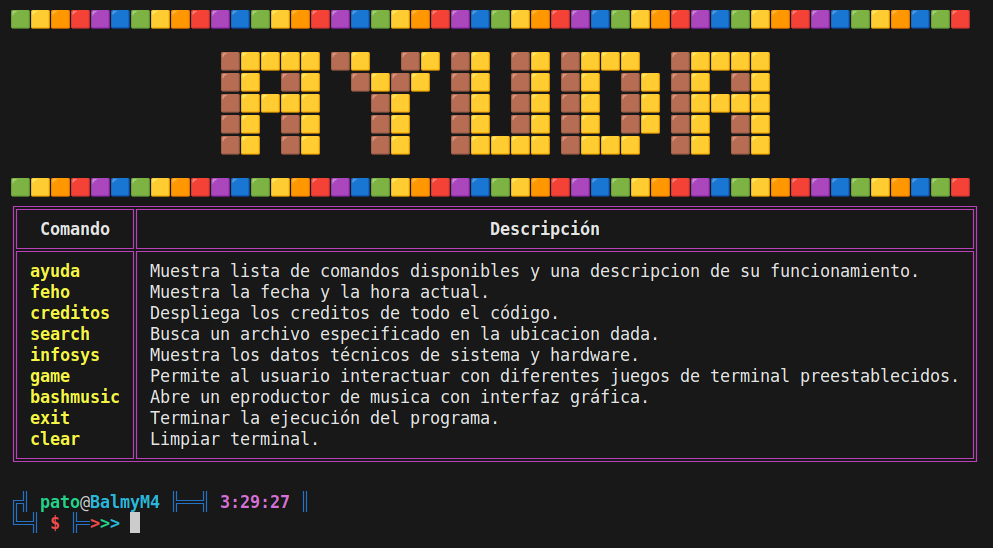
\includegraphics[width=0.7\textwidth]{ayuda.png}
    \caption{Ejecución del comando \textbf{ayuda}:}
    \label{fig:ejemplo}
\end{figure}

% creditos -----------------------------------------------
\noindent
\textbf{Comando:} \verb|creditos|. \\
\textbf{Descripción:} despliega una tabla que contiene los créditos del proyecto. El comando es puramente visual, por lo que el código se basa exclusivamente en print's y echo's que imprimen la decoración.

\begin{figure}[H]
    \centering
    
\includegraphics[width=0.65\textwidth]{creditos.png}
    \caption{Ejecución del comando \textbf{creditos}:}
    \label{fig:ejemplo}
\end{figure}

% FEH0 -----------------------------------------------
\newpage
\noindent
\textbf{Comando:} \verb|feho|. \\
\textbf{Descripción:} acrónimo de fecha y hora, el comando muestra la hora y fecha actual. Esta información se obtiene del archivo /proc/driver/rtc, el cual contiene información sobre el real time clock del sistema. Su funcionamiento consiste en identificar los datos rtc time y rtc date en el archivo con el comando grep, para posteriormente guardar los datos con awk en una variable local.\\

\noindent
\textbf{Código:}
\begin{lstlisting}
hora=$(grep "rtc_time" /proc/driver/rtc | awk '{print $3}')
IFS=":" read -ra time <<< "$hora"
hour=${time[0]}
min=${time[1]}
sec=${time[2]}


fecha=$(grep "rtc_date" /proc/driver/rtc | awk '{print $3}')
IFS="-" read -ra date <<< "$fecha"
year=${date[0]}
month=${date[1]}
day=${date[2]}
\end{lstlisting}

\begin{figure}[H]
    \centering
    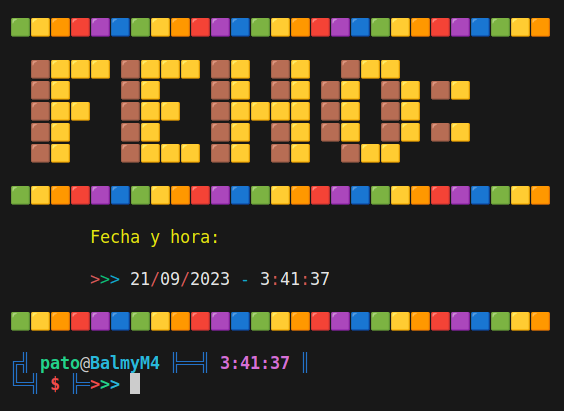
\includegraphics[width=0.9\textwidth]{feho.png}
    \caption{Ejecución del comando \textbf{feho}:}
    \label{fig:ejemplo}
\end{figure}

% search -----------------------------------------------
\newpage
\noindent
\textbf{Comando:} \verb|search|. \\
\textbf{Descripción:} al escribir el comando te redirige a un apartado donde se te piden dos parámetros, el nombre del archivo a buscar y la ruta donde se va a buscar. Si la ruta dada no es absoluta, el programa lo detecta y cambia a un modo automático de ruta relativa partiendo de HOME.\\

\noindent
\textbf{Código:}
\begin{lstlisting}
if [ -e "$ruta/$archivo"  ]; then
    echo -e "\n\t${v}El archivo se ha encontrado con exito."
    echo -e "\n\t${am}Listado de la ruta: ${b}"
    ls $ruta

elif [ -e "$HOME/$ruta/$archivo" ]; then
    echo -e "\n\t${v}El archivo se ha encontrado con exito."
    echo -e "\n\t${am}Listado de la ruta: ${b}"
    ls $HOME/$ruta
else
    echo -e "\n\t${r}El archivo no se ha encontrado."
fi
\end{lstlisting}

\begin{figure}[H]
    \centering
    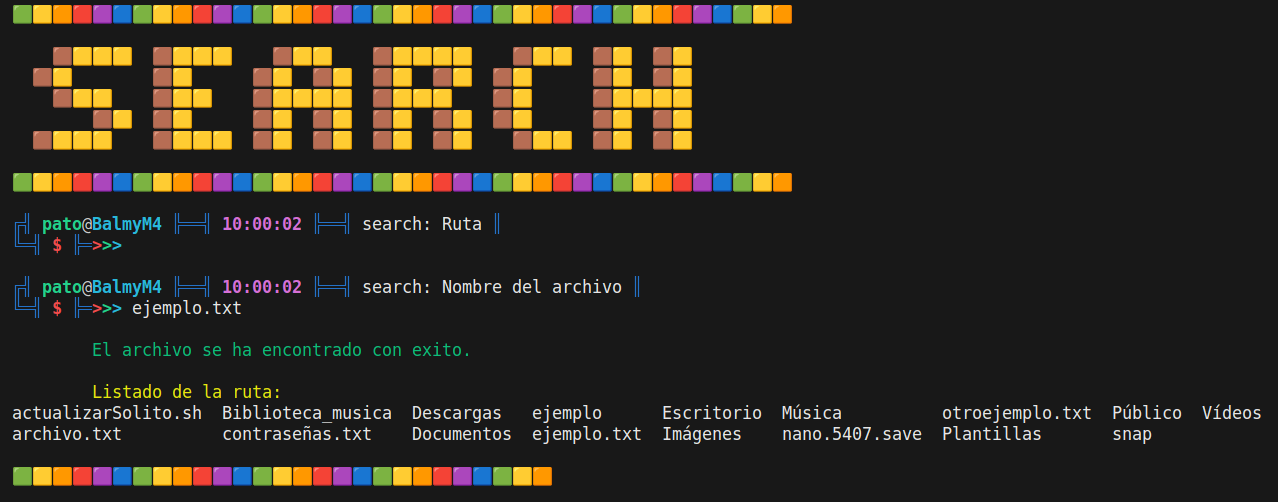
\includegraphics[width=1\textwidth]{search.png}
    \caption{Ejecución del comando \textbf{search}:}
    \label{fig:ejemplo}
\end{figure}

% infosys -----------------------------------------------
\newpage
\noindent
\textbf{Comando:} \verb|infosys|. \\
\textbf{Descripción:} muestra algunos datos técnicos del sistema operativo y de hardware, para ello se utilizó variables de entorno, el comando grep, awk y algunos otros para obtener la información de los archivos necesarios. En la figura 5 se observan todos los datos que muestra el comando.\\

\noindent
\textbf{Fragmento del código:}
\begin{lstlisting}
show_info() {
    echo -e "\e[1m$1 \e[0m$2"
}

show_info "Sistema:             " "$(uname -s)"
show_info "Hostname:            " "$HOSTNAME"
show_info "Kernel:              " "$(uname -r)"

\end{lstlisting}

\begin{figure}[H]
    \centering
    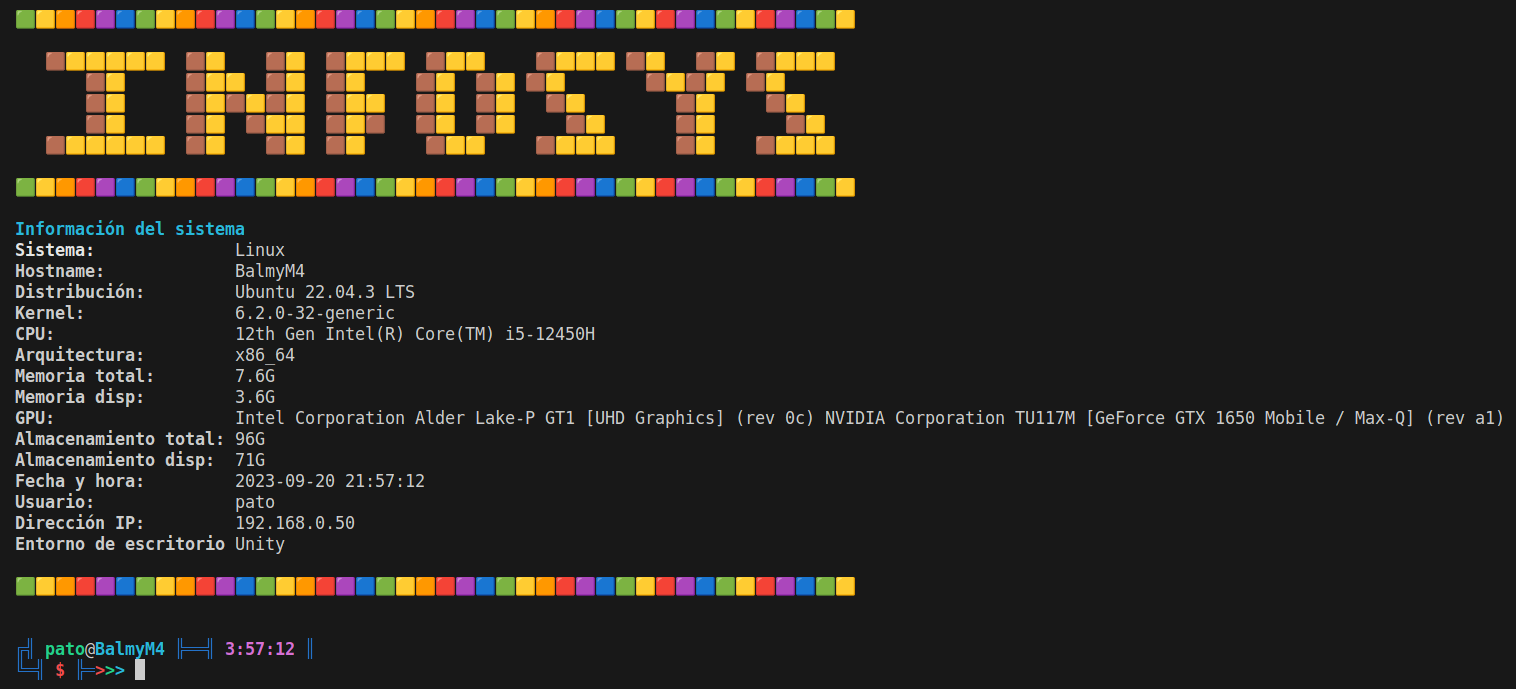
\includegraphics[width=0.9\textwidth]{infosys.png}
    \caption{Ejecución del comando \textbf{infosys}:}
    \label{fig:ejemplo}
\end{figure}

% game -----------------------------------------------
\newpage
\noindent
\textbf{Comando:} \verb|game|. \\
\textbf{Descripción:} al ejecutar el comando se redirige a un apartado de selección de minijuegos. Hay tres minijuegos disponibles, el segundo es el típico piedra papel o tijeras en el cual se escogerá aleatoriamente la opción del oponente. El primer minijuego consiste en adivinar un número seleccionado aleatoriamente a través de pistas que se te irán dando. El último minijuego consiste en resolver cinco laberintos disponibles. 

\begin{figure}[H]
    \centering
    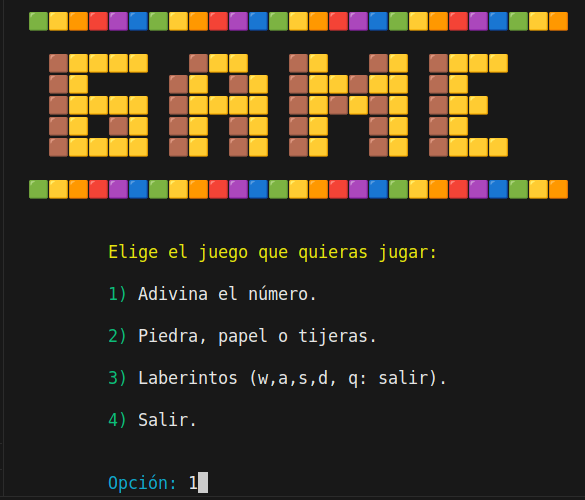
\includegraphics[width=0.7\textwidth]{game.png}
    \caption{Ejecución del comando \textbf{game}:}
    \label{fig:ejemplo}
\end{figure}

% bashmusic -----------------------------------------------
\noindent
\textbf{Comando:} \verb|bashmusic|. \\
\textbf{Descripción:} El comando bashmusic permite al usuario reproducir archivos de musica que se tengan almacenados en un directorio dado. El script muestra un menu de opciones (vease Fig.~ \ref{fig:ejemplo0}) que permite al usuario cambiar entre directorios y hacer 3 direfentes tipos de reproduccioón: \\Reproduccion de una pista de audio (Fig.~ \ref{fig:ejemplo1}).\\Reproducción de todas las pistas de audio contenidas en el directorio seleccionado (Fig.~ \ref{fig:ejemplo2}).\\Reproducir todas las pistas de audio contenidas en el directorio seleccionado en modo aleatorio (Fig.~ \ref{fig:ejemplo3}).\\Una vez que una pista está en reproducción, se despliega una tabla de controles que detalla los atajos para diferentes acciones como: Pausa/Reproducir, siguiente pista, pista anterior, mostrar playlist, repetir pista, repetir playlist y detener reproducción. Finalmente el script permite al usuario terminar su ejecucion con un comando numerico (5).           

\begin{figure}[H]
    \centering
    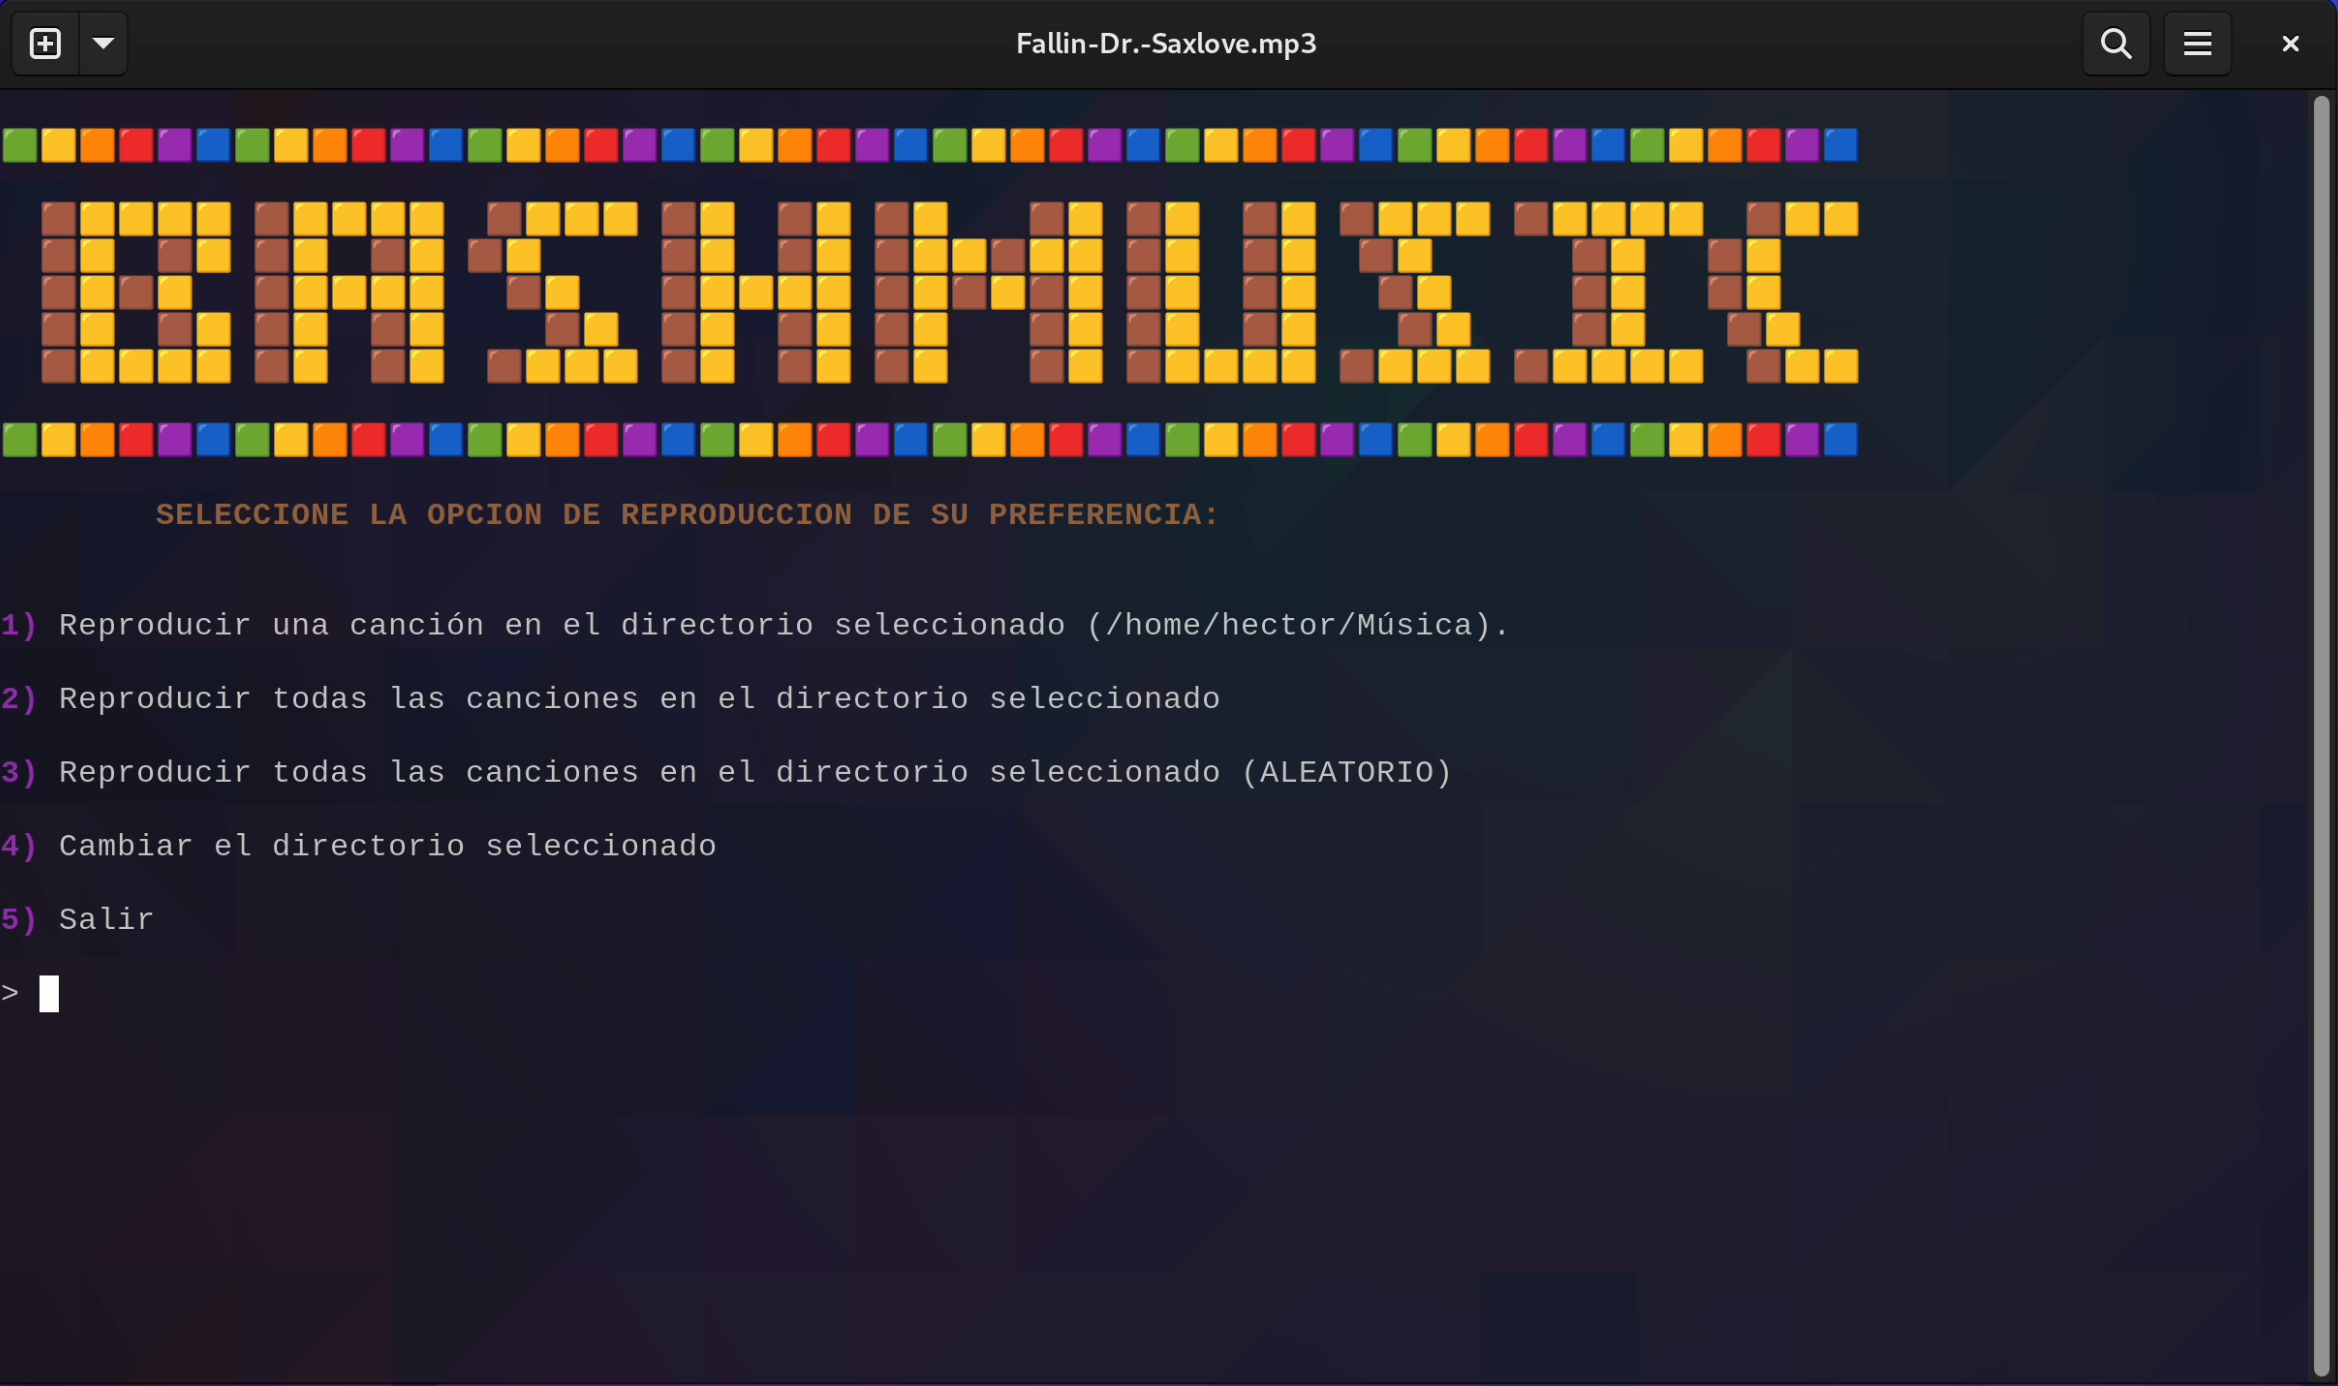
\includegraphics[width=0.9\textwidth]{bashmusic_mp.png}
    \caption{Menu principal \textbf{bashmusic}:}
    \label{fig:ejemplo0}
\end{figure}

\begin{figure}[H]
    \centering
    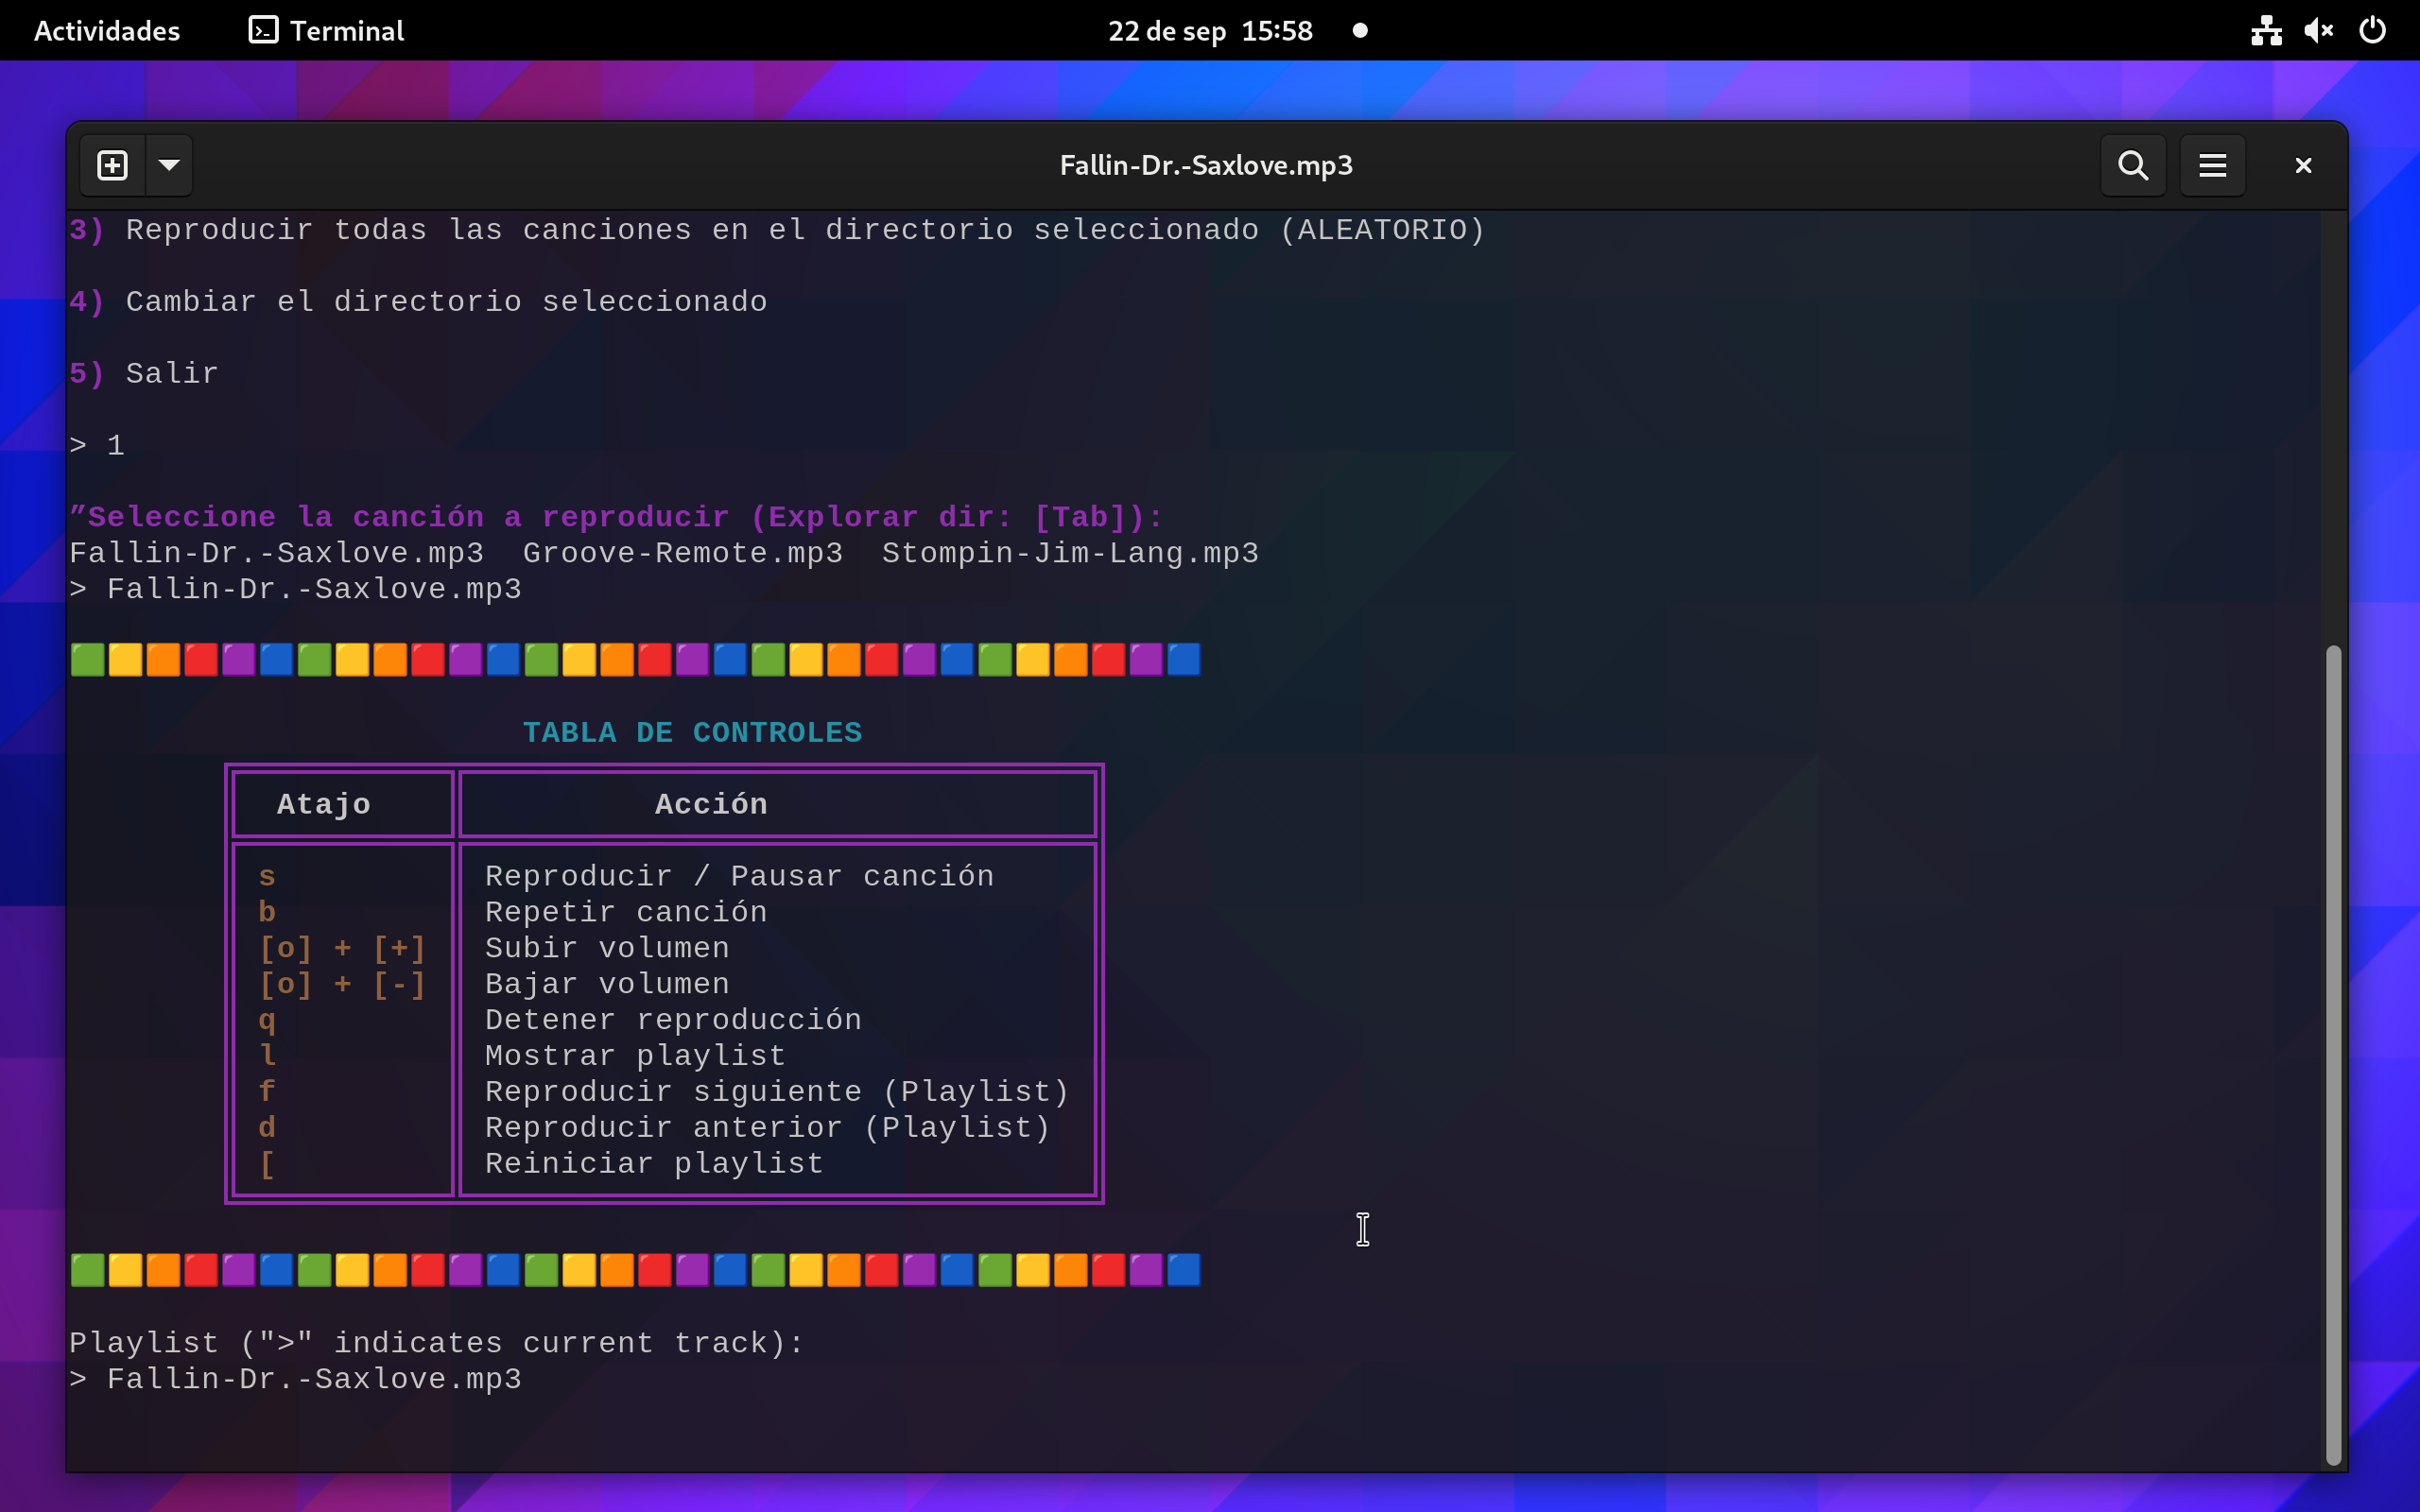
\includegraphics[width=0.9\textwidth]{bashmusic_1.png}
    \caption{Opción 1:  \textbf{Reproducción de pista.}}
    \label{fig:ejemplo1}
\end{figure}

\begin{figure}[H]
    \centering
    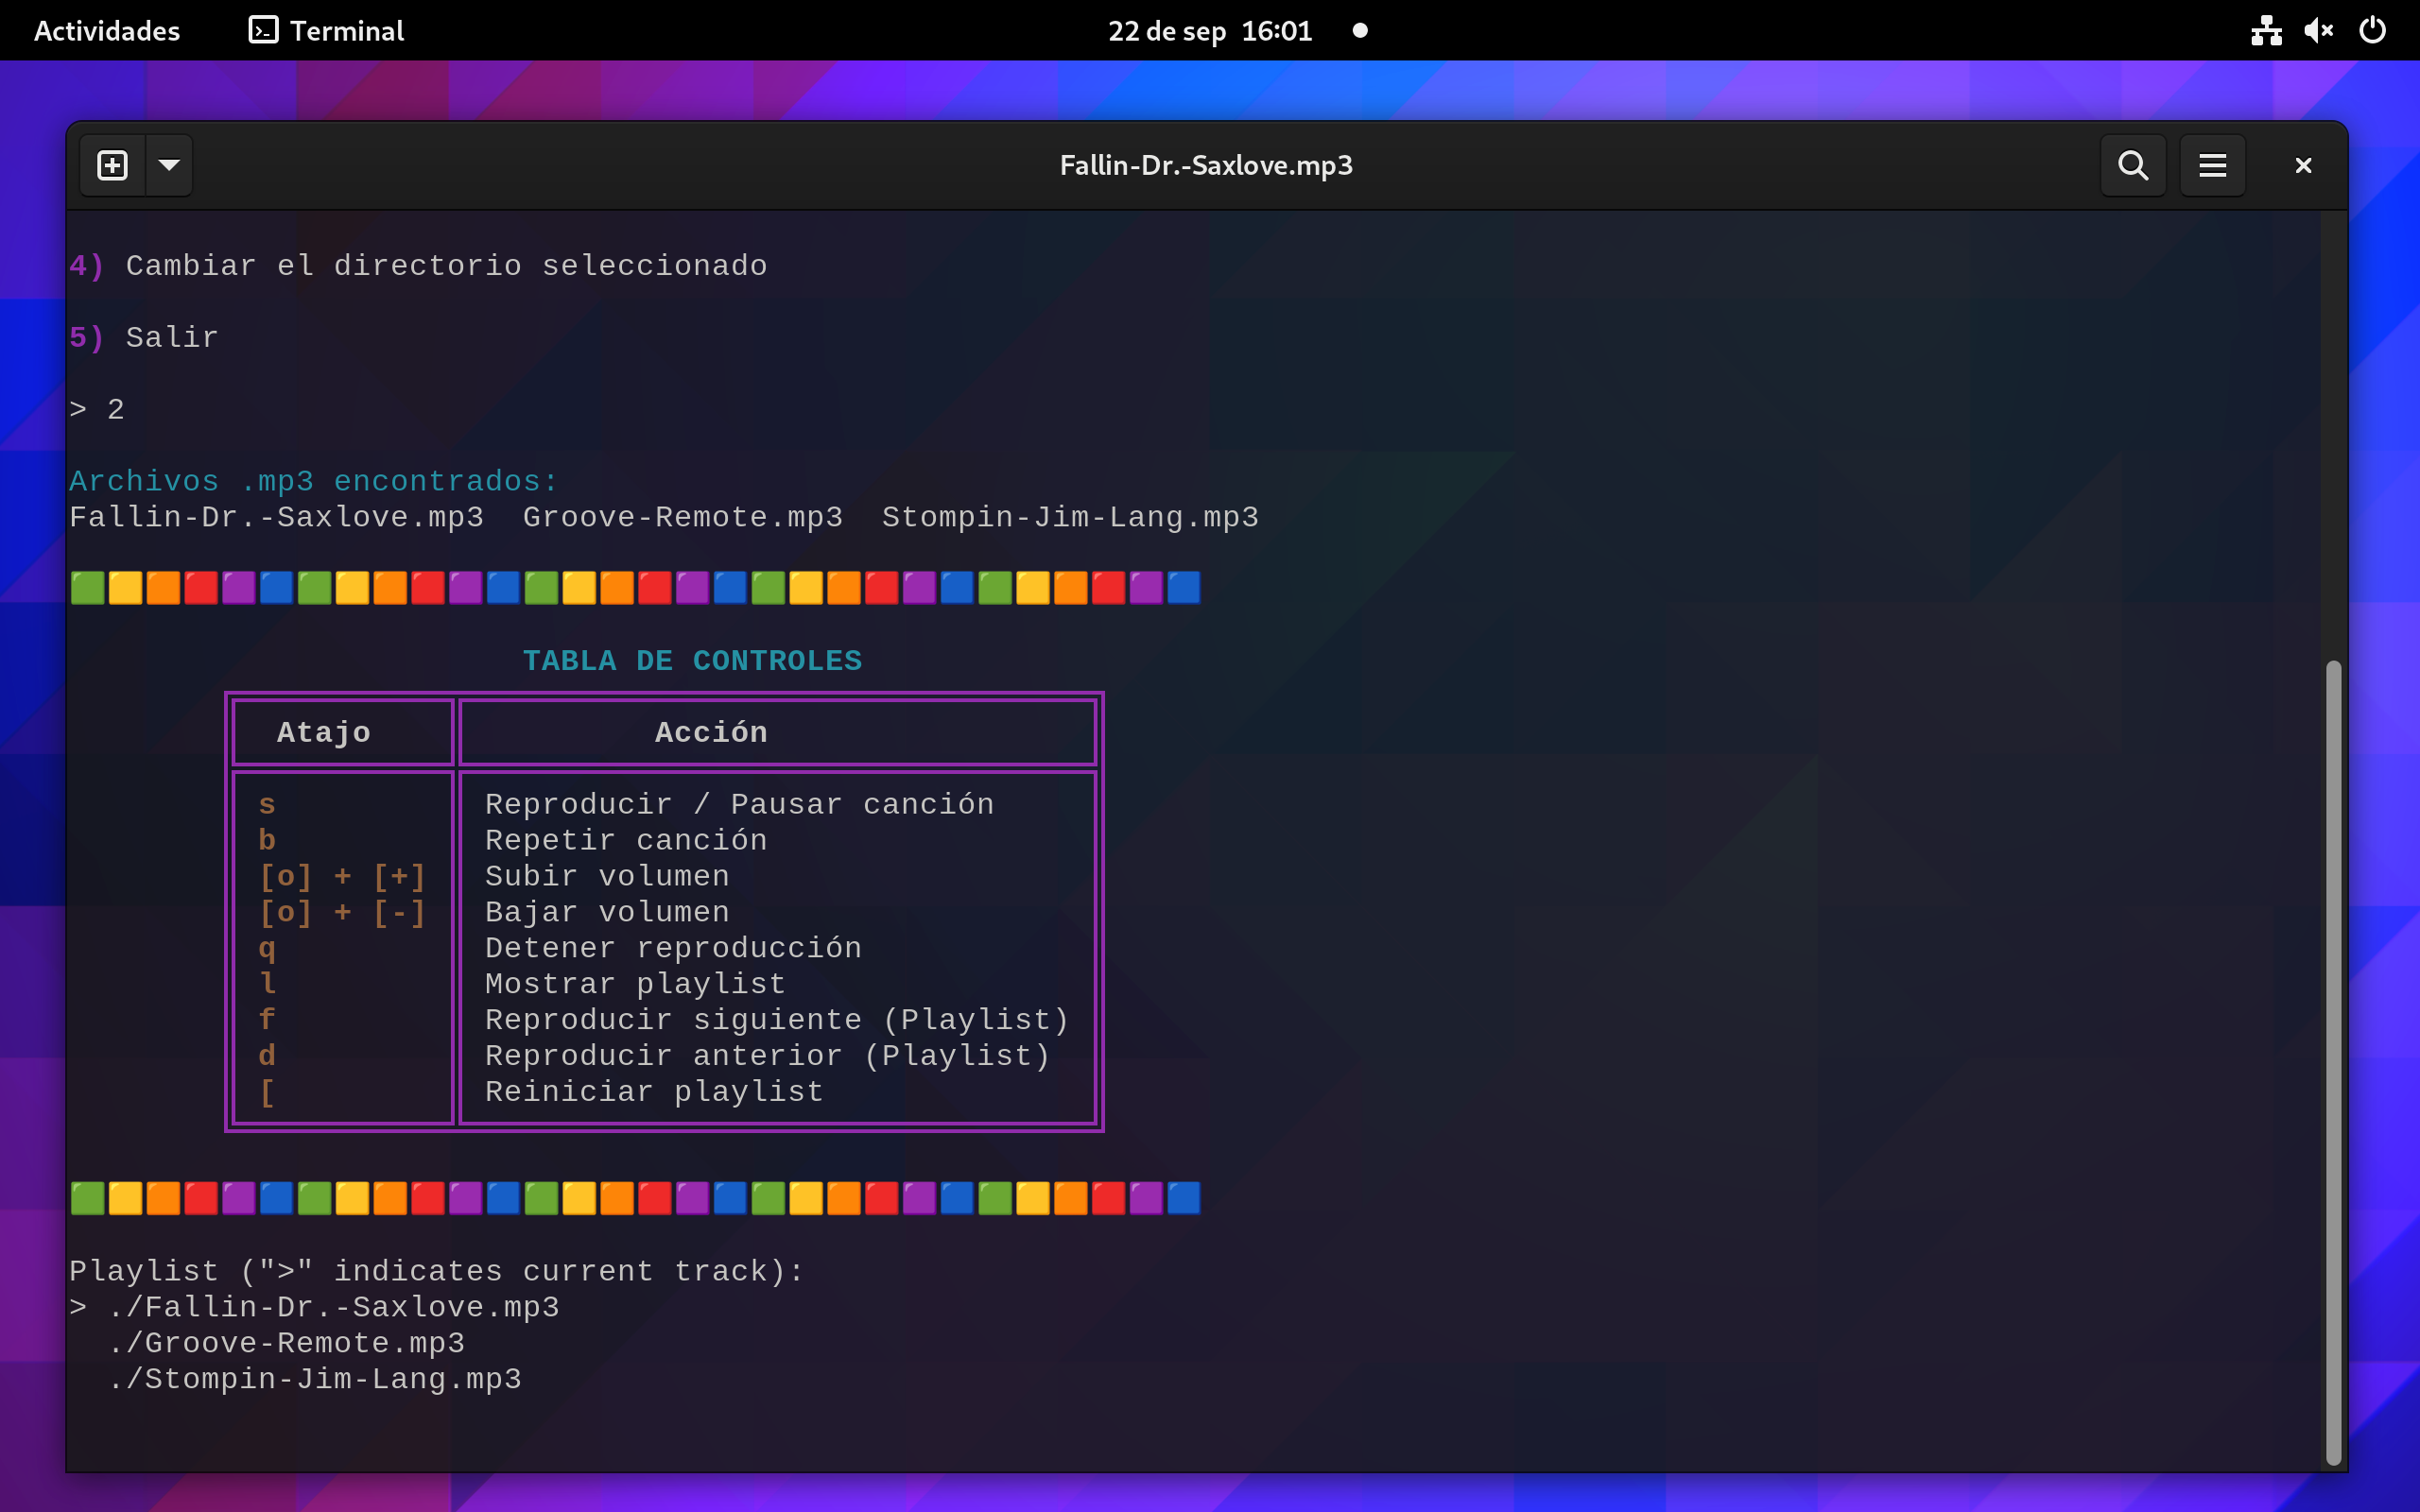
\includegraphics[width=0.9\textwidth]{bashmusic_2.png}
    \caption{Opción 2:  \textbf{Reproducir todas las pistas en el directorio seleccionado.}}
    \label{fig:ejemplo2}
\end{figure}

\begin{figure}[H]
    \centering
    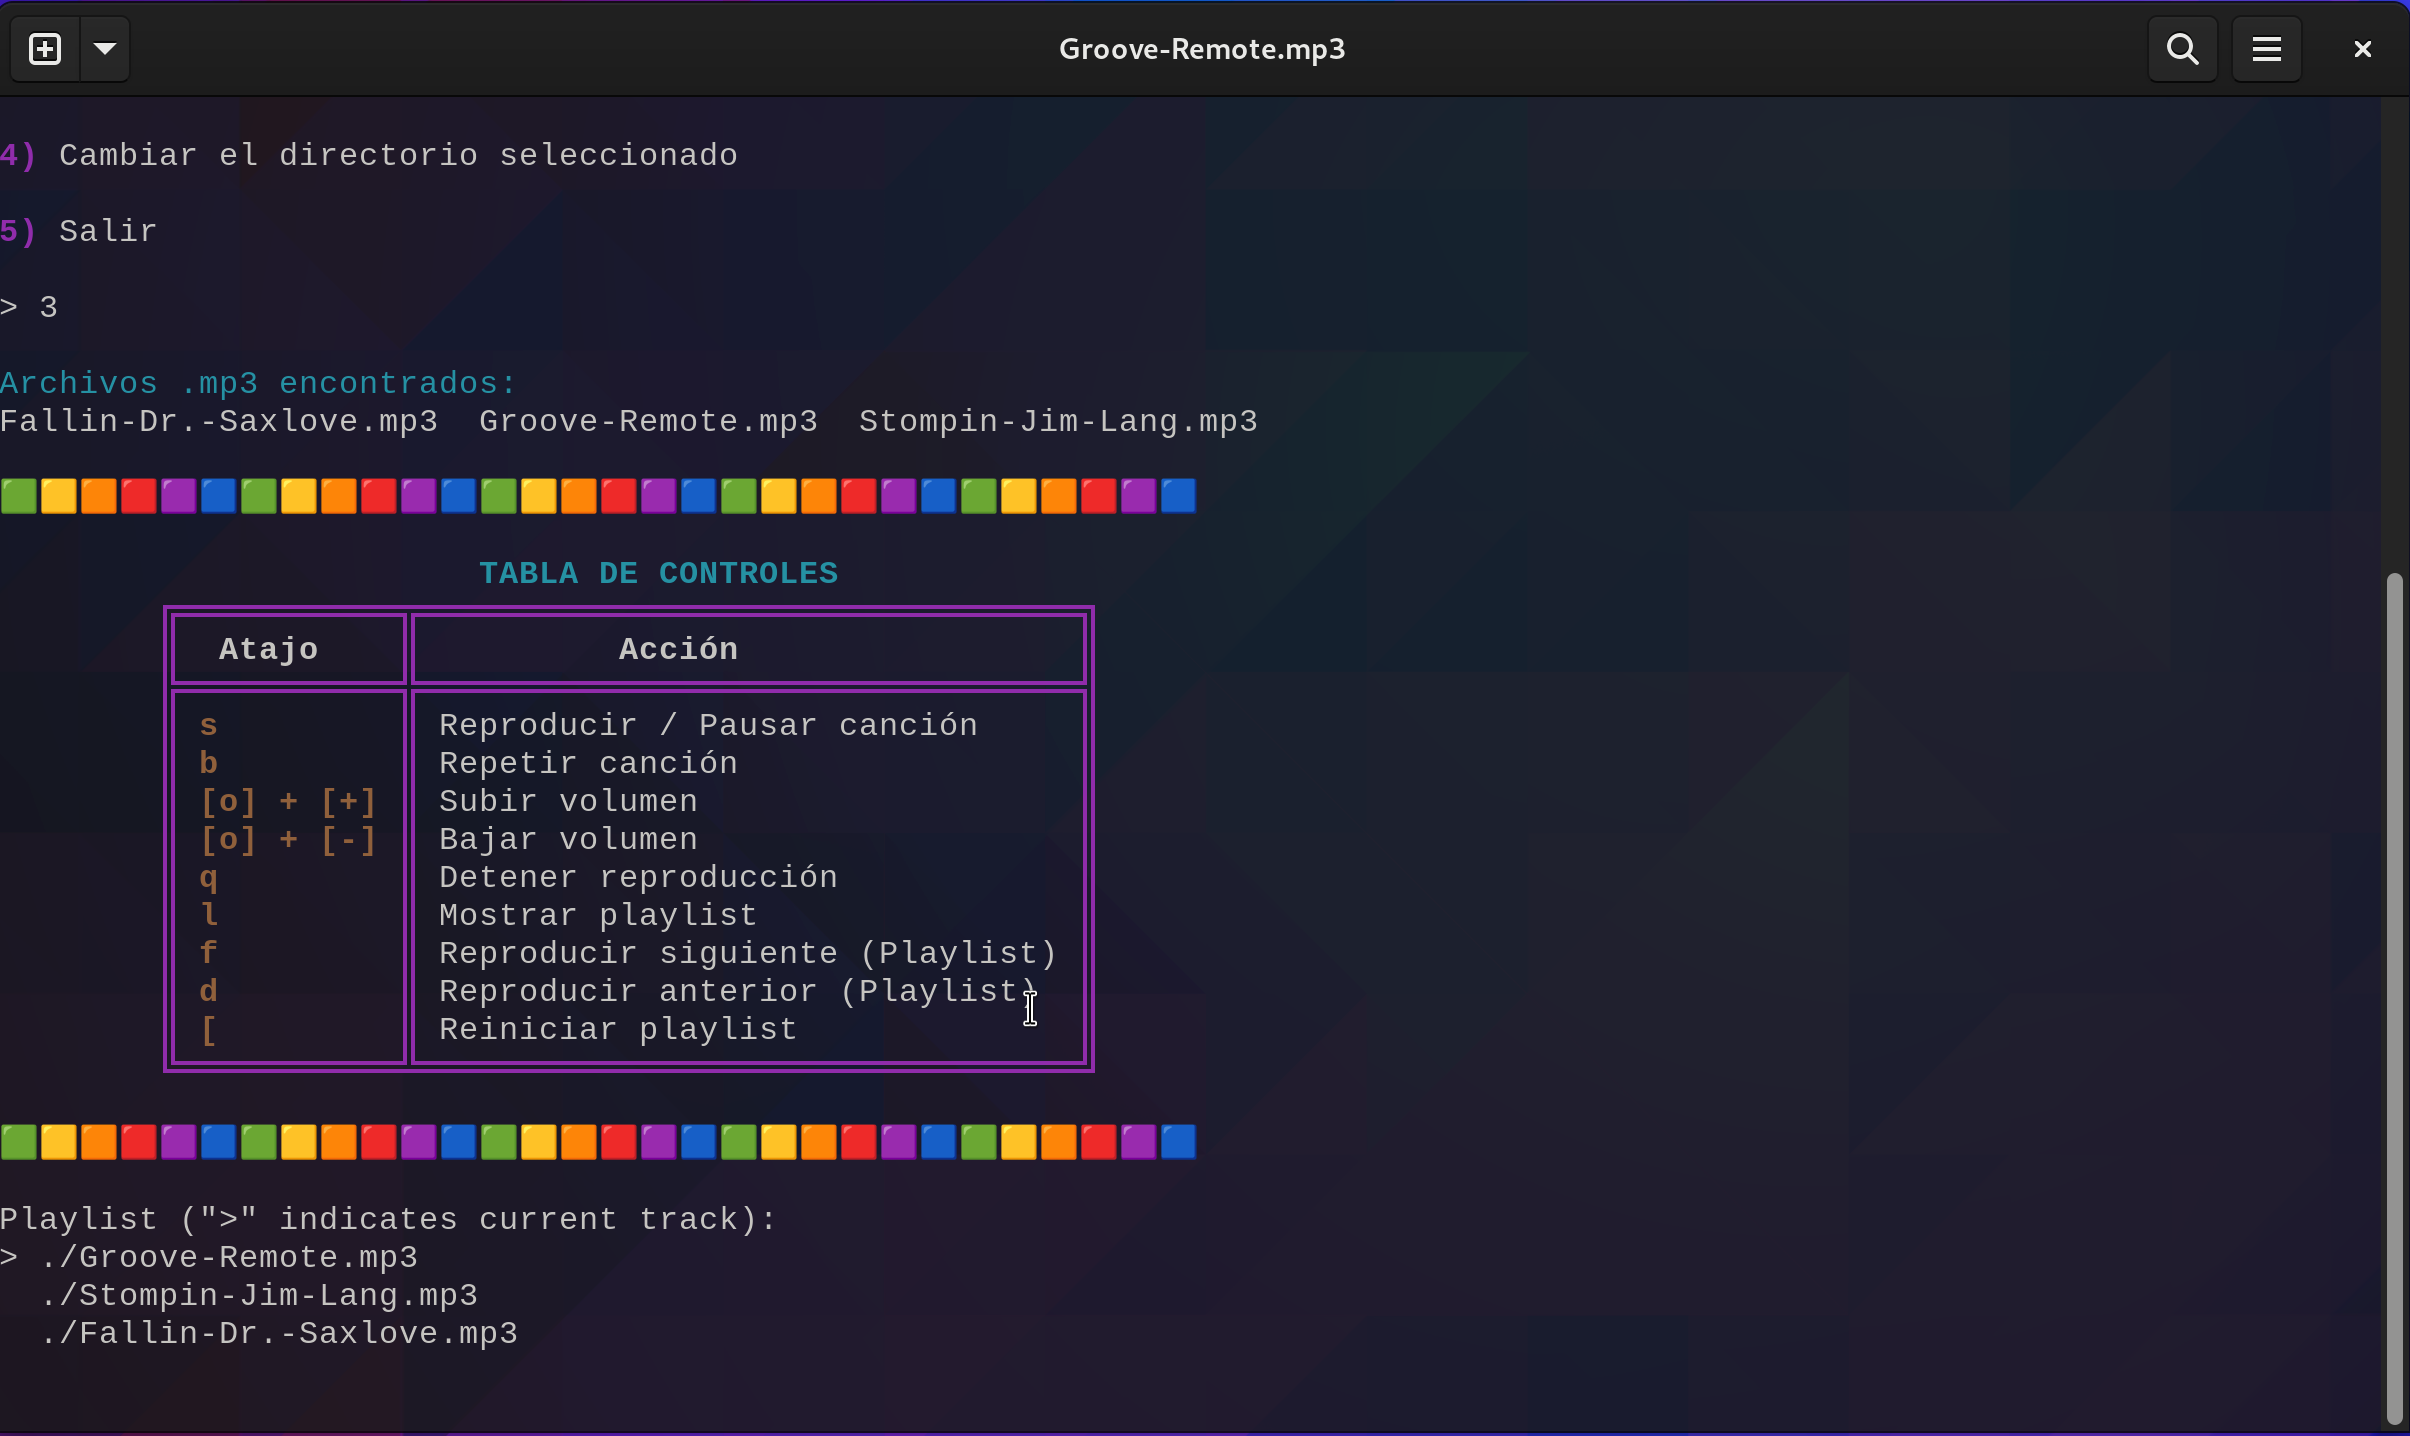
\includegraphics[width=0.9\textwidth]{bashmusic_3.png}
    \caption{Opción 3:  \textbf{Reproducir todas las pistas en el directorio seleccionado (Aleatorio).}:}
    \label{fig:ejemplo3}
\end{figure}

\begin{figure}[H]
    \centering
    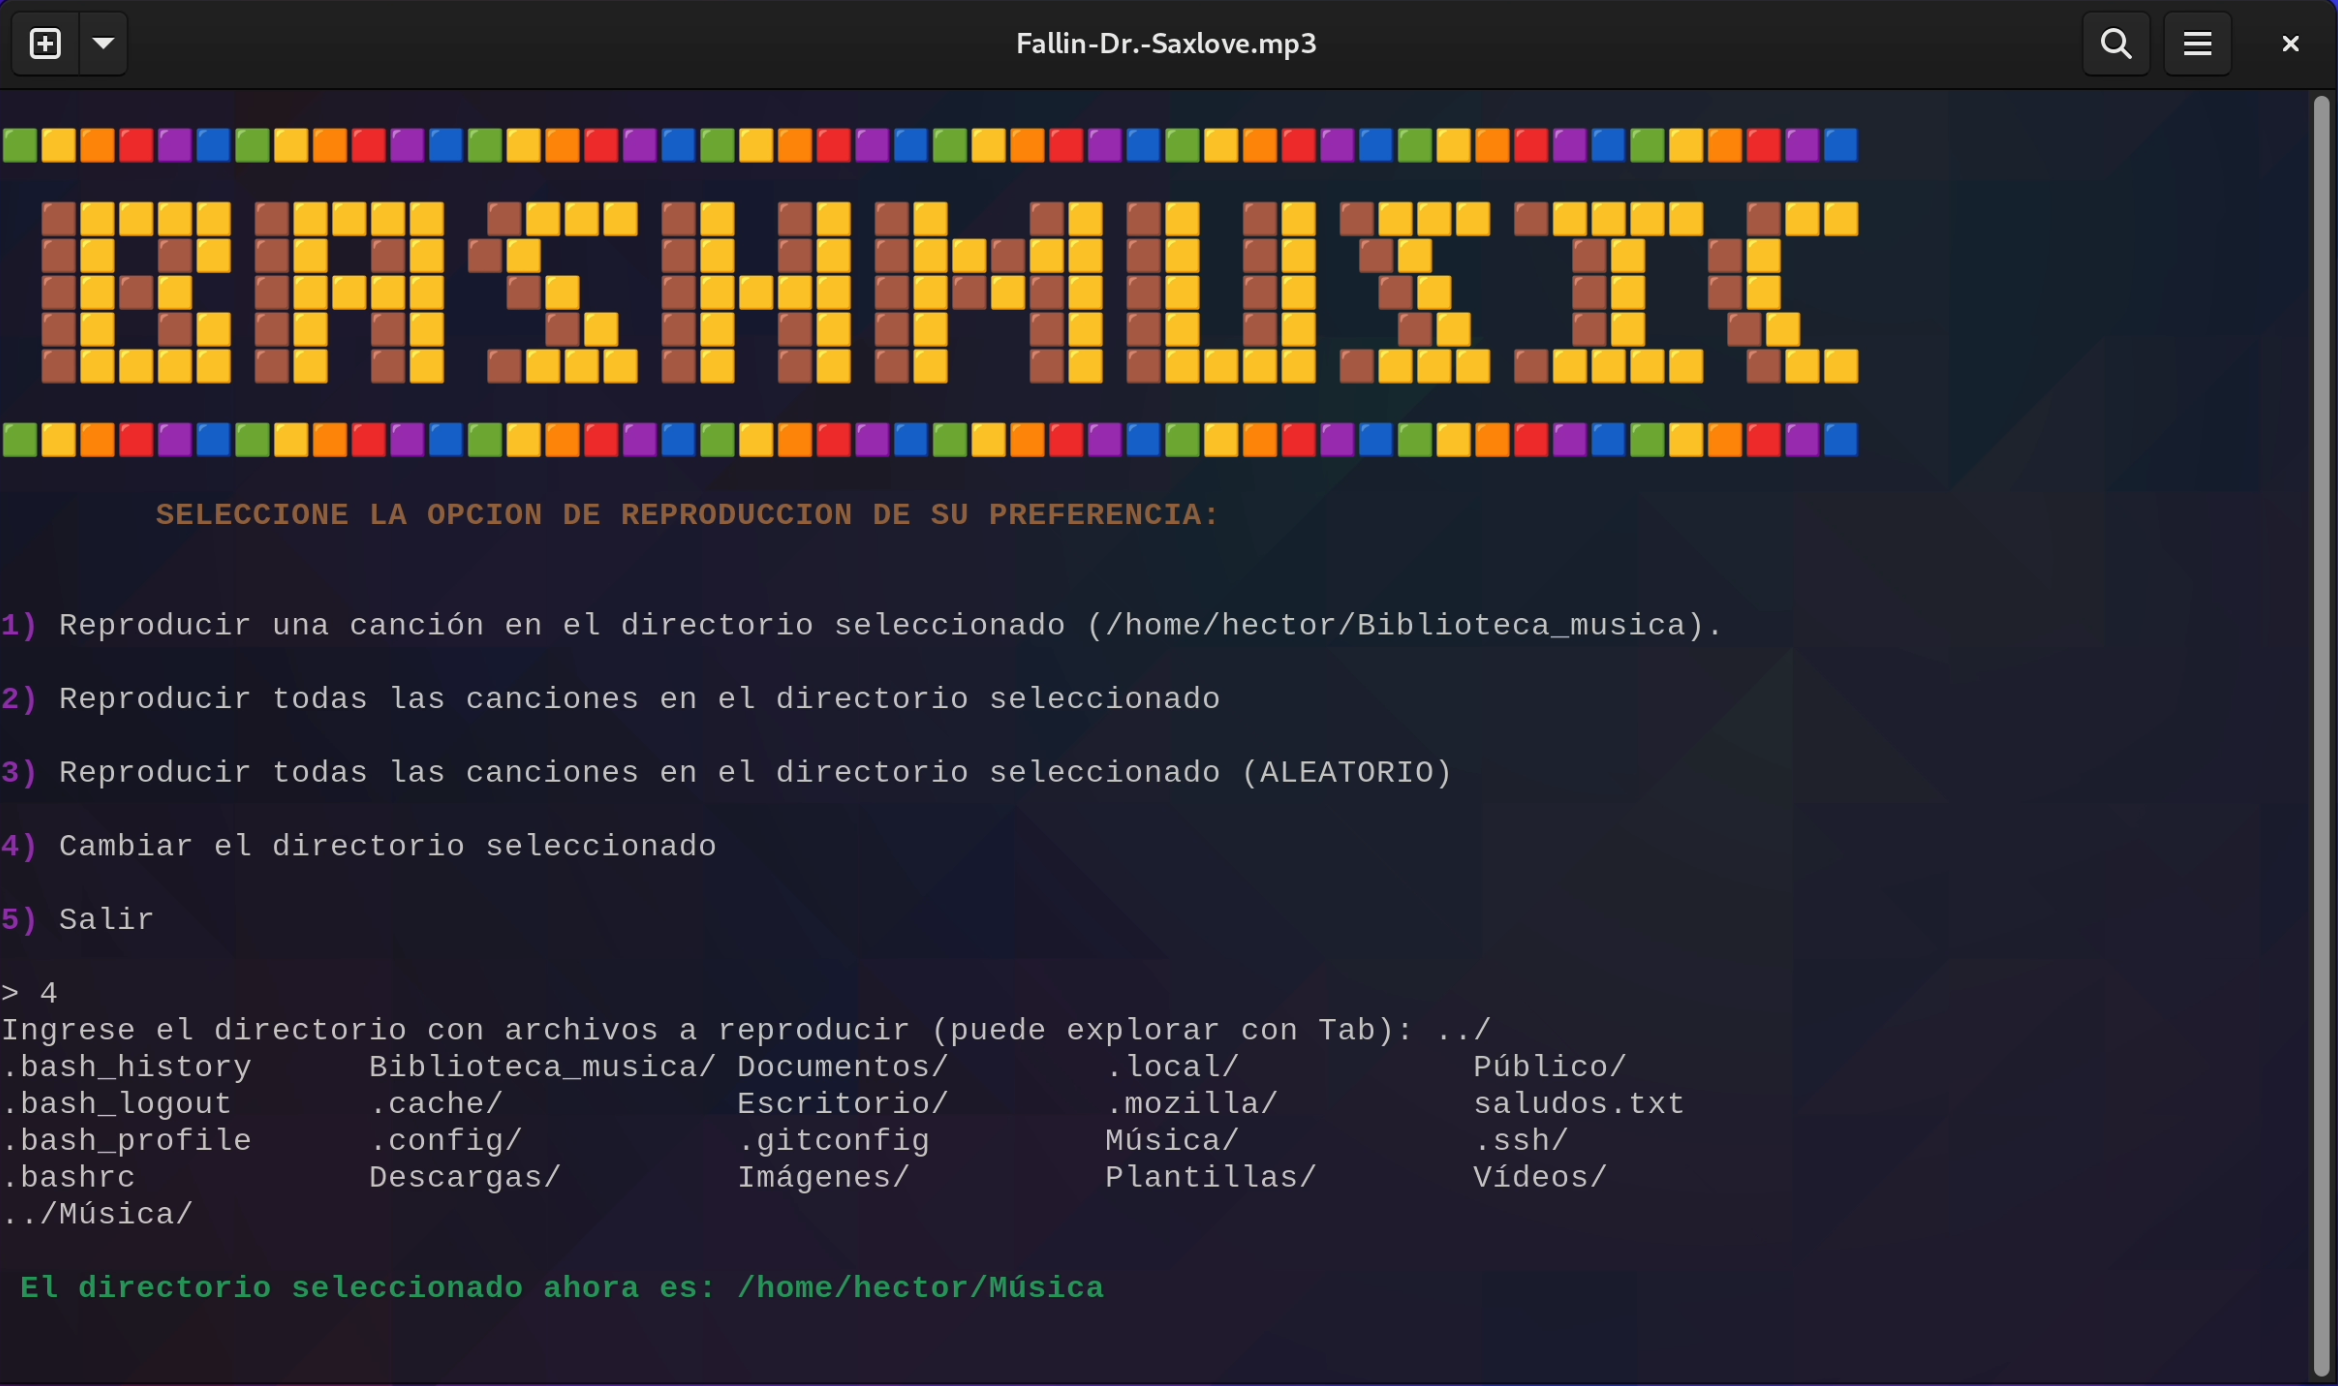
\includegraphics[width=0.9\textwidth]{bashmusic_4.png}
    \caption{Opción 3:  \textbf{Cambiar el directorio seleccionado.}}
    \label{fig:ejemplo4}
\end{figure}

% exit -----------------------------------------------
\noindent
\textbf{Comando:} \verb|exit|. \\
\textbf{Descripción:} termina la ejecución del programa.           

\begin{figure}[H]
    \centering
    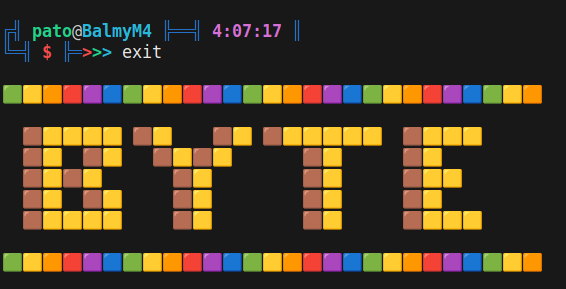
\includegraphics[width=0.9\textwidth]{exit.png}
    \caption{Ejecución del comando \textbf{exit}:}
    \label{fig:ejemplo}
\end{figure}
 

%============================================================================
\newpage
\section{Conclusiones}
\textbf{Hector Manuel Larios Ponce}:\\En conclusión y bajo mi perspectiva personal, el desarrollo de este proyecto de bash script ha sido un éxito y ha demostrado ser una herramienta valiosa para abordar las bases que todo profesional de las tecnologías de la información debe tener para garantizar un óptimo desempeño el ámbito profesional. A través de la implementación de este script, hemos logrado la automatización de tareas y conocer mas a fondo el sistema de archivos que maneja un sistema Linux. La flexibilidad de Bash como lenguaje de scripting ha permitido una personalización eficiente y una fácil adaptación a las demandas del presente proyecto.\\Durante el proceso de desarrollo, hemos enfrentado desafíos que han impulsado nuestras habilidades de programación y resolución de problemas. Hemos aprendido a mejorar continuamente el código para garantizar su funcionamiento robusto y confiable.\\Además, el trabajo en equipo y la colaboración desempeñaron un papel fundamental en el éxito de este proyecto. La comunicación efectiva y la asignación de tareas nos permitieron avanzar de manera eficiente y superar obstáculos.
\\\\

\textbf{Gabriel Patricio Balam Flores}:\\Los objetivos generales que se plantearon para este proyecto se han cumplido con éxito. Este proyecto fue algo exigente y nos ayudó a fortalecer algunas habilidades de investigación y de programación tanto en bash script como en nuestra lógica para resolver problemas. Claramente algunas partes del proyecto fueron más demandantes que otras, pero con una buena asignación de tareas y trabajo en equipo se pudo disolver la carga de trabajo hasta el punto que casi no se sintió.
En lo personal creo que el aprendizaje que te deja un proyecto como este es muy grande y sienta las bases para empezar a desarrollar proyectos más ambiciosos a futuro. Aunque algunas partes del código son mejorables y la experiencia de cara al usuario se puede pulir mucho más, pienso que para el tiempo asignado el producto final es satisfactorio, ya que cumple con todas las especificaciones que se nos dieron. De tener más tiempo, creo que se podría haber hecho una experiencia más limpia e intuitiva para los usuarios.


\end{document}
